% Options for packages loaded elsewhere
\PassOptionsToPackage{unicode}{hyperref}
\PassOptionsToPackage{hyphens}{url}
%
\documentclass[
]{article}
\usepackage{lmodern}
\usepackage{amssymb,amsmath}
\usepackage{ifxetex,ifluatex}
\ifnum 0\ifxetex 1\fi\ifluatex 1\fi=0 % if pdftex
  \usepackage[T1]{fontenc}
  \usepackage[utf8]{inputenc}
  \usepackage{textcomp} % provide euro and other symbols
\else % if luatex or xetex
  \usepackage{unicode-math}
  \defaultfontfeatures{Scale=MatchLowercase}
  \defaultfontfeatures[\rmfamily]{Ligatures=TeX,Scale=1}
\fi
% Use upquote if available, for straight quotes in verbatim environments
\IfFileExists{upquote.sty}{\usepackage{upquote}}{}
\IfFileExists{microtype.sty}{% use microtype if available
  \usepackage[]{microtype}
  \UseMicrotypeSet[protrusion]{basicmath} % disable protrusion for tt fonts
}{}
\makeatletter
\@ifundefined{KOMAClassName}{% if non-KOMA class
  \IfFileExists{parskip.sty}{%
    \usepackage{parskip}
  }{% else
    \setlength{\parindent}{0pt}
    \setlength{\parskip}{6pt plus 2pt minus 1pt}}
}{% if KOMA class
  \KOMAoptions{parskip=half}}
\makeatother
\usepackage{xcolor}
\IfFileExists{xurl.sty}{\usepackage{xurl}}{} % add URL line breaks if available
\IfFileExists{bookmark.sty}{\usepackage{bookmark}}{\usepackage{hyperref}}
\hypersetup{
  hidelinks,
  pdfcreator={LaTeX via pandoc}}
\urlstyle{same} % disable monospaced font for URLs
\usepackage{graphicx}
\makeatletter
\def\maxwidth{\ifdim\Gin@nat@width>\linewidth\linewidth\else\Gin@nat@width\fi}
\def\maxheight{\ifdim\Gin@nat@height>\textheight\textheight\else\Gin@nat@height\fi}
\makeatother
% Scale images if necessary, so that they will not overflow the page
% margins by default, and it is still possible to overwrite the defaults
% using explicit options in \includegraphics[width, height, ...]{}
\setkeys{Gin}{width=\maxwidth,height=\maxheight,keepaspectratio}
% Set default figure placement to htbp
\makeatletter
\def\fps@figure{htbp}
\makeatother
\setlength{\emergencystretch}{3em} % prevent overfull lines
\providecommand{\tightlist}{%
  \setlength{\itemsep}{0pt}\setlength{\parskip}{0pt}}
\setcounter{secnumdepth}{-\maxdimen} % remove section numbering

\author{}
\date{}

\begin{document}

\hypertarget{stage-m2r}{%
\section{Stage M2R}\label{stage-m2r}}

Greg McShane 2020

\href{https://macbuse.github.io/}{my webpage}

\hypertarget{bounds-and-statistics-for-closed-geodesics}{%
\section{Bounds and statistics for closed
geodesics}\label{bounds-and-statistics-for-closed-geodesics}}

\hypertarget{context}{%
\subsection{Context}\label{context}}

Consider an orientable surface \(\Sigma\) with negative Euler
characteristic, a minimal set of generators of the fundamental group,
and a constant curvature -1 metric on \(\Sigma\). Each free homotopy
class C of closed oriented curves on S determines three numbers: 1. the
word length (that is, the minimal number of letters needed to express
\(\gamma\) as a cyclic word in the generators and their inverses), 1.
the minimal geometric self-intersection number 1. the geometric length
\(\ell(\gamma)\) ie the length of the unique closed geodesic in the
class \(\gamma\).

These three numbers can be explicitly computed (or approximated) using a
computer so we can do experiments and check results algorithmically.

From a theoretical point of view :

\begin{itemize}
\tightlist
\item
  The relation between word length and geometric length was studied by
  Milnor in the 60s then Policott and Sharp from a statistical point of
  view in the 90s.
\item
  The relation between intersection number and geometric length was
  studied by Basmajian about 10 years ago then by Chis and her coathors
  from a statistical point of view.
\end{itemize}

\begin{center}\rule{0.5\linewidth}{0.5pt}\end{center}

The principal (non statistical) results are easy to state precisely. Let
\(\gamma\) be a cyclically reduced word in the fundamental group and
\(\ell(\gamma)\) the length of the unique closed geodesic representing
this conjucacy class then :

Milnor proved that there is a constant \(K\) which depends on the metric
such that \[(1/K) |\gamma| < \ell(\gamma) < K|\gamma|. \] where
\(|\gamma|\) is the word length and \(\ell(\gamma)\) the length of the
curve for the \emph{choice} of metric.

Likewise Basmajian proved that there is a constant \(K\) which depends
on the metric such that
\[(1/K) i(\gamma,\gamma) < \ell(\gamma) < K i(\gamma,\gamma). \] where
\(i(\gamma,\gamma)\) is the geometric intersection number.

The way that the factor \(K\) varies carries important geometric
information.

\begin{center}\rule{0.5\linewidth}{0.5pt}\end{center}

\hypertarget{details-of-the-stage}{%
\subsubsection{Details of the stage}\label{details-of-the-stage}}

We will review the basic geometric constructions and in particular the
work of Milnor which relates combinatorial group theory to Riemannian
geometry. Then we will study Basmajian'method for obtaining inequalities
relating intersection number to length. We will look at the applications
of this to giving effective bounds in Scott's Theorem on simple lifts.
Finally we will study the methods required by Lalley and Chis to obtain
the statistical relation between length and intersection number.

\begin{figure}
\centering
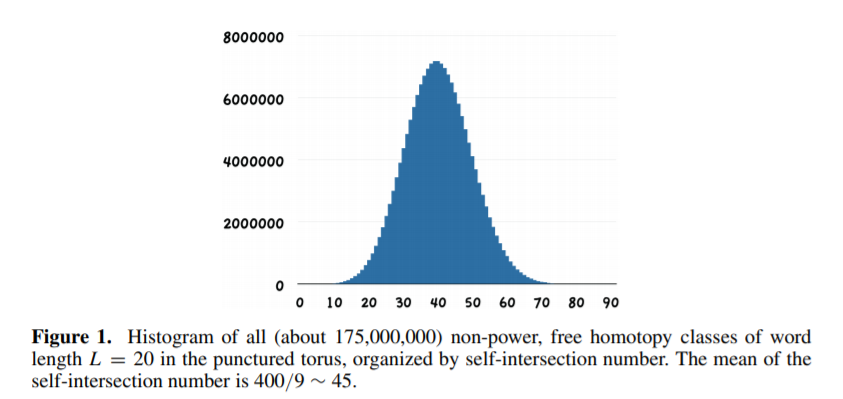
\includegraphics{./chas.png}
\caption{img}
\end{figure}

\begin{center}\rule{0.5\linewidth}{0.5pt}\end{center}

\hypertarget{references}{%
\subsubsection{References}\label{references}}

\begin{enumerate}
\def\labelenumi{\arabic{enumi}.}
\tightlist
\item
  Relations between Word Length, Hyperbolic Length and Self-Intersection
  Number of Curves on Surfaces, Moira Chis
  \href{http://www.math.stonybrook.edu/~moira/papers/2015ChisRelations_between_Word_Length_Hyperbolic_Length_and_Self-Intersection_Number_of_Curves_on_Surfaces.pdf}{manuscript}
\item
  M. Pollicott and R. Sharp, Comparison theorems and orbit counting in
  hyperbolic geometry. Trans. Amer. Math. Soc. 350, 473499, 1998.
\item
  Universal length bounds for non-simple closed geodesics on hyperbolic
  surfaces Ara Basmajian Journal of Topology, Volume 6, Issue 2, June
  2013, Pages 513--524, https://doi.org/10.1112/jtopol/jtt005
\item
  Self-intersections in combinatorial topology: statistical structure
  Moira Chis, Steven P. Lalley
  \href{https://arxiv.org/abs/1012.0580}{arxiv}
\item
  Short closed geodesics with self-intersections Viveka Erlandsson and
  Hugo Parlier \href{https://arxiv.org/pdf/1609.00217.pdf}{arxiv}
\item
  Building hyperbolic metrics suited to closed curves and applications
  to lifting simply, Tarik Aougab, Jonah Gaster, Priyam Patel, Jenya
  Sapir \href{https://arxiv.org/abs/1603.06303}{arxiv}
\item
  Peter Scott. Subgroups of surface groups are almost geometric. J.
  London Math. Soc. (2) 17(1978)
\end{enumerate}

\href{https://github.com/macbuse/MATH/edit/master/stage\%20m2r\%202020_bis.md}{web
page}

\end{document}
